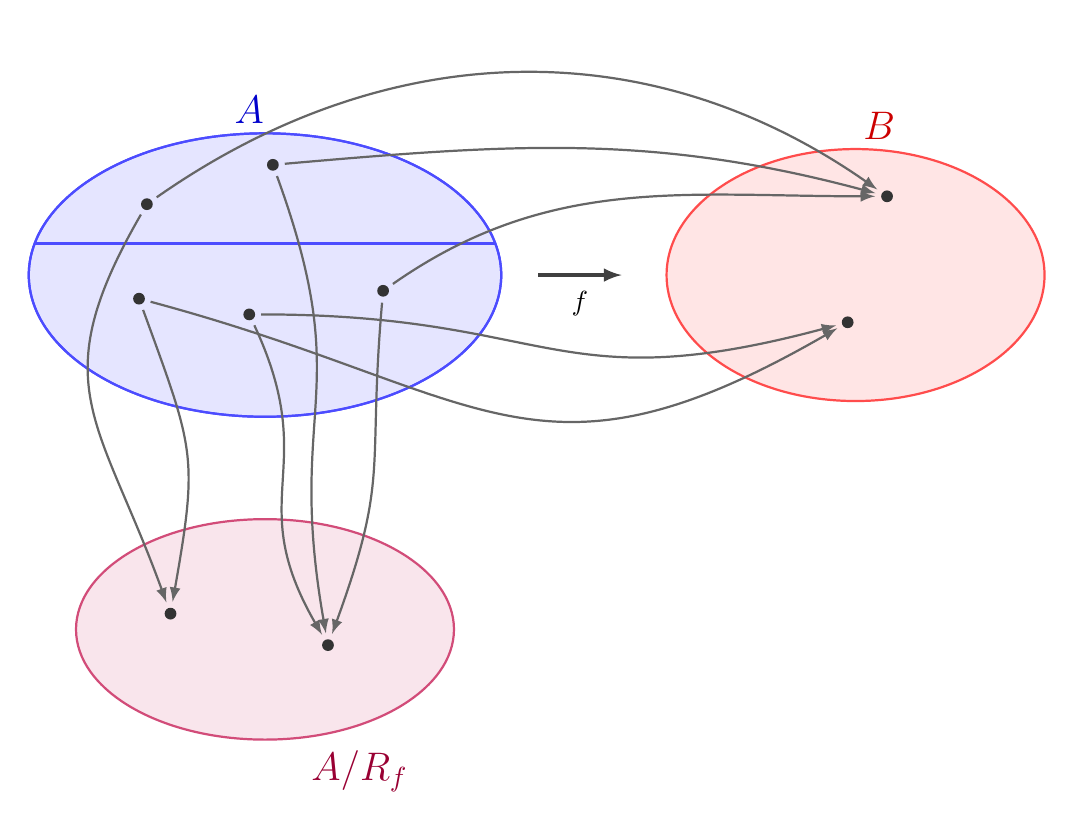
\begin{tikzpicture}[>=latex]

% --- Global TikZ Styles for Consistency ---
\tikzset{
    setA/.style={fill=blue!10, draw=blue!70, thick},
    setB/.style={fill=red!10, draw=red!70, thick},
    setC/.style={fill=purple!10, draw=purple!70, thick}, % Nieuwe stijl voor A/R_f
    labelA/.style={text=blue!80!black, font=\Large\bfseries},
    labelB/.style={text=red!80!black, font=\Large\bfseries},
    labelC/.style={text=purple!80!black, font=\Large\bfseries},
    partition/.style={draw=blue!70, thick},
    point/.style={circle, fill=black!80, inner sep=1.5pt},
    arrow/.style={
        ->,
        >=latex,
        thick,
        draw=black!60, % Iets donkerder gemaakt voor de vele overlappende lijnen
        shorten >=2pt,
        shorten <=2pt
    },
    mainarrow/.style={
        ->,
        >=latex,
        very thick,
        draw=black!75,
        shorten >=2pt,
        shorten <=2pt
    }
}

% --- Verzameling A (Boven Links) ---
\path[setA] (0, 0) ellipse (3.0cm and 1.8cm);
\node[labelA] at (-0.2, 2.1) {$A$};

% Partition Line clipped inside A
\begin{scope}
    \clip (0, 0) ellipse (3.0cm and 1.8cm);
    \draw[partition] (-3.2, 0.4) -- (3.2, 0.4);
\end{scope}

% Redraw border of A so clipping does not visually affect the outline
\draw[blue!70, thick] (0, 0) ellipse (3.0cm and 1.8cm);

% Punten in A
\node[point] (p1) at (-1.5, 0.9) {};  % linksboven
\node[point] (p2) at (0.1, 1.4) {};   % middenboven
\node[point] (p3) at (-1.6, -0.3) {}; % linksonder
\node[point] (p4) at (-0.2, -0.5) {}; % middenonder
\node[point] (p5) at (1.5, -0.2) {};  % rechtsonder

% --- Verzameling B (Boven Rechts) ---
% Iets hoger en naar rechts geplaatst zoals in de screenshot
\path[setB] (7.5, 0.0) ellipse (2.4cm and 1.6cm);
\node[labelB] at (7.8, 1.9) {$B$};

% Punten in B
\node[point] (b1) at (7.9, 1.0) {}; % Bovenste punt
\node[point] (b2) at (7.4, -0.6) {}; % Onderste punt

% --- Verzameling A/R_f (Onder Links) ---
\path[setC] (0, -4.5) ellipse (2.4cm and 1.4cm);
\node[labelC] at (1.2, -6.3) {$A/R_f$};

% Punten in A/R_f
\node[point] (q1) at (-1.2, -4.3) {}; % Linker punt
\node[point] (q2) at (0.8, -4.7) {};  % Rechter punt

% --- Pijlen en Mapping ---

% Hoofdpijl f (tussen A en B)
\draw[mainarrow] (3.4, 0.0) -- (4.6, 0.0) node[midway, below=2pt] {$f$};

% Pijlen van A naar B (Horizontale stroom)
\draw[arrow] (p1) to[out=35, in=145, looseness=1.0] (b1);
\draw[arrow] (p2) to[out=5,  in=165, looseness=1.0] (b1);
\draw[arrow] (p3) to[out=-15, in=210, looseness=1.3] (b2);
\draw[arrow] (p4) to[out=0,  in=195, looseness=1.3] (b2);
\draw[arrow] (p5) to[out=35, in=180] (b1); % Deze kronkelt mooi omhoog

% Pijlen van A naar A/R_f (Verticale stroom)
\draw[arrow] (p1) to[out=-120, in=110, looseness=1.3] (q1);
\draw[arrow] (p3) to[out=-70, in=80, looseness=1.3] (q1);
\draw[arrow] (p2) to[out=-70, in=100, looseness=1.3] (q2);
\draw[arrow] (p4) to[out=-65, in=120, looseness=1.3] (q2);
\draw[arrow] (p5) to[out=-95, in=70, looseness=1.3]  (q2);

\end{tikzpicture}